%% Author_tex.tex
%% V1.0
%% 2012/13/12
%% developed by Techset
%%
%% This file describes the coding for rsproca.cls

\documentclass[]{rsos}%%%%where rsos is the template name


\usepackage[T1]{fontenc}
\usepackage[utf8]{inputenc}


% tightlist command for lists without linebreak
\providecommand{\tightlist}{%
  \setlength{\itemsep}{0pt}\setlength{\parskip}{0pt}}

% From pandoc table feature
\usepackage{longtable,booktabs,array}
\usepackage{calc} % for calculating minipage widths
% Correct order of tables after \paragraph or \subparagraph
\usepackage{etoolbox}
\makeatletter
\patchcmd\longtable{\par}{\if@noskipsec\mbox{}\fi\par}{}{}
\makeatother
% Allow footnotes in longtable head/foot
\IfFileExists{footnotehyper.sty}{\usepackage{footnotehyper}}{\usepackage{footnote}}
\makesavenoteenv{longtable}



%%%% *** Do not adjust lengths that control margins, column widths, etc. ***

%%%%%%%%%%% Defining Enunciations  %%%%%%%%%%%
\newtheorem{theorem}{\bf Theorem}[section]
\newtheorem{condition}{\bf Condition}[section]
\newtheorem{corollary}{\bf Corollary}[section]
%%%%%%%%%%%%%%%%%%%%%%%%%%%%%%%%%%%%%%%%%%%%%%%

\begin{document}


%%%% Article title to be placed here
\title{A systematic machine learning approach to quantifying coverage and representation bias in population estimates from mobile phone app data}

\author{
Carmen Cabrera$^{1}$,
Francisco Rowe$^{1}$}

\address{
  $^{1}$Geographic Data Science Lab, Department of Geography and Planning, University of Liverpool, Liverpool, United Kingdom.\\
  $^{}$}
%%%% Subject entries to be placed here %%%%
\subject{
Mobile phone data,
Human mobility,
Explainable AI,
Spatial analysis}

%%%% Keyword entries to be placed here %%%%
\keywords{
Mobile phone data,
Human mobility,
Location,
Explainable AI,
Spatial analysis}

%%%% Insert corresponding author and its email address}
\corres{
  Carmen Cabrera\\
  e-mail: \href{mailto:C.Cabrera@liverpool.ac.uk}{\nolinkurl{C.Cabrera@liverpool.ac.uk}}
}

%%%% Abstract text to be placed here %%%%%%%%%%%%
\begin{abstract}
Traditional data sources such as censuses and surveys are costly, infrequent, and often unavailable in crisis-affected regions. User location data derived from GPS-enabled mobile phone (MP) applications offer near-real-time, high-resolution insights into population distribution, but unequal access to and use of mobile technologies introduces biases that threaten representativeness. Existing bias assessments typically require demographic attributes, which are often unavailable, and focus on national-level estimates. We present a generalisable framework to measure and explain biases in aggregated MP app data without the need for individual-level demographic data. The framework quantifies coverage bias, which relates to the share of the population captured, at national and subnational levels, evaluates spatial heterogeneity and clustering, and models the geographic variation of bias as a function of area-based covariates using explainable machine learning. We illustrate the framework using four MP app datasets for the UK, aligned with the 2021 national census. We find that MP data consistently achieve higher coverage than major national surveys, though bias varies spatially and by data source. Multi-application datasets generally reduce (?) coverage bias relative to single-application sources. X emerges as a consistent and important factor in determining the local magnitude of coverage bias.
\end{abstract}
%%%%%%%%%%%%%%%%%%%%%%%%%%%

\providecommand{\EndFirstPage}{%
}

\maketitle

\newpage

\section{Introduction}\label{introduction}

Traditional data streams, such as the census and surveys have been the
primary official source to provide a comprehensive representation of
national populations in countries worldwide. However, fast-paced
societal changes and emergency disasters, such as climate-induced
hazards and COVID-19 have tested and accentuated weaknesses in
traditional data systems \citep{green2021}. Traditional data systems often
provide data in infrequent and coarse temporal and geographical
resolutions \citep{rowe23-bigdata}. Generally they are expensive to maintain
and operate, and are slow taking months or years since they data are
collected to their release \citep{rowe23-bigdata}. Data collection from
climate- or conflict-impacted areas is generally unfeasible because of
restrictions due to high levels of insecurity and risk
\citep{iradukunda2025}. Yet, fast-paced societal changes require high
frequency, granular and up-to-date information to support real-time
planning, policy and decision making.

At the same time, we have seen the confluence of two diverging trends in
data availability. On the one hand, growing evidence of declining survey
response rates across many countries over the last 20 years is
accumulating \textbf{{[}REF{]}}. Dwindling numbers in surveys can represent
distorted picture of society \textbf{{[}REF{]}}. On the other hand, significant
advances in sensor technology, computational power, storage and digital
network platforms have unleashed a data revolution producing large
trails of digital trace data \textbf{{[}REF{]}}. These data are now routinely
collected and stored. They offer spatially granular, frequent and
instant information to capture and understand human activities at
unprecedentedly high resolution and scale, with the potential to produce
real-time actionable intelligence to support decision making \textbf{{[}REF{]}}.
Hence, national statistical offices are actively seeking to integrate
these data into their national data infrastructure \textbf{{[}REF{]}}.

Mobile phone data (MPD) collected via GPS- and IP-based technology have
become a prominent source of nontraditional data to monitor population
changes. Increasing usage of mobile services on smartphones and wearable
devices have resulted in the generation of large volumes of geospatial
data, offering novel opportunities to advance understanding of spatial
human behaviour, and thus revolutionise research, business and
government decision making and practices \citep{rowe23-bigdata}. MPD are now
a core component of the digital economy, creating new market
opportunities for data intelligence businesses, such as Cuebiq/Spectus,
Safegraph and Locomizer. They have been used to create critical evidence
to support policy making, prominently during the COVID-19 pandemic. In
research, MPD have been used to develop innovative approach to infer
mode of transport {[}REF{]}, monitor footfall changes {[}REF{]}, profile daily
mobility signatures {[}REF{]}, sense land use patterns {[}REF{]}, predict
socioeconomic levels {[}REF{]}, define urban extents {[}REF{]}, quantify tourism
activity {[}REF{]} and estimate migration and population displacement {[}REF{]}.

However, the use of MPD present major epistemological, methodological
and ethical challenges \citep{rowe23-bigdata}. A key unresolved challenge is
potential biases in MPAD compromising their statistical
representativeness and perpetuate social injustice {[}REF{]}. Biases reflect
societal digital and socioeconomic inequalities. Biases emerge from
differences in the access and use of the mobile phone applications used
to collect MPD \citep{wesolowski13-biases}. Only a fraction of the population
in a geographical area owns a smartphone, and even an smaller share
actively uses a specific mobile phone app. In the UK, for example, 98\%
of the adult population have a mobile phone and 92\% of this population
use a smartphone \citep{ofcom23}, but a smaller percentage actively use
Facebook (70\%) or Twitter (23\%) \citep{statista24}. Additionally, biases
emerge from differences in the access and use of digital technology
across population subgroups reflecting socioeconomic and demographic
disparities. For instance, wealthy, young and urban populations
generally have greater access and more intensively use of mobile phone
applications, and therefore tend to be over-represented in MPD {[}REF{]}.

The use of biased MPD can thus have major practical and societal
implications. If used uncorrected, MPD reproduce selective patterns of
smartphone ownership and application usage, rendering inaccurate or
distorted representations of human population activity. Such
representations disproportionately reflect behaviours of younger, urban
and higher-income users while underrepresenting marginalised or
less-connected groups. Distorted representations based on biased MPD can
thus misguide decision making, policy and planning interventions, and
thus amplify existing socio-economic disparities. In practice, existing
applications of MPD often use uncorrected population statistics derived
from MPD and have thus been constrained to offer a partial picture for a
limited segment of the overall population. Such data can only afford to
provide rough signals about the spatial distribution of (e.g.~spatial
concentration), trends (e.g.~increasing) and changes (e.g.~low to high)
in populations \citep{rowe22-sensing-ukraine}. They have cannot provide a
full representation of the overall population.

Efforts have been made to measure and assess biases in aggregate
population counts from digital data sources. Existing analyses typically
measure the extent of bias measuring the system-wide difference in the
representation of population counts from digital platforms and censuses.
To estimate the representation of digital data sources, the penetration
rate is computed as the active user base of a digital platform over the
census resident population. Existing analyses have thus been able to
established systematic gender, age and socio-economic biases in
population data obtained via API (or Application Programming Interface)
from social media platforms, such as Facebook and Twitter/X. However,
this approach requires information on the demographic and socio-economic
attributes of the collected sample and has focused on estimating biases
at the country level. Yet, these attributes are generally unavailable
for MPD, and biases may vary widely across subnational areas. What is
missing is an systematic approach to measure biases in population counts
from digital platforms, when population attributes are unknown, and
quantify the geographic variability in the extent of biases in these
data.

To address this gap, this paper aims to establish a standardised
approach to empirically measure the extent of biases in population data
derived from digital platforms, and identify their key underlying
contextual factors across subnational areas. We seek to address the
following research questions:

\begin{itemize}
\tightlist
\item
  What is the comparative extent of population coverage of digital
  sources relative to widely-used traditional surveys?
\item
  How systematic is the association between larger biases and the
  over-representation of rural, more deprived, child and elderly
  populations?
\item
  To what extent, are population data assembled from multiple
  applications versus single applications associated with lower bias?
\end{itemize}

Our approach proposes a statistical indicator of population coverage to
measure the extent of bias, and uses explainable machine learning to
identify key contextual factors contributing to spatial variations in
the extent of bias. Biases in digital trace data can emerge from
multiple sources, such as algorithmic changes, device duplication and
geographic location accuracy {[}REF{]}. We do not intend to identify these
individual sources of error. We focus on quantifying the extent of
``cumulative'\,' bias; that is, the resulting bias from the accumulation
of these error sources. We use data collected from single and multiple
mobile phone apps, and compare their results. As outlined above, we test
the extent to which biases can be mitigated by leveraging information
from multiple apps encompassing a more diverse user population.
Specifically, we use two single-app (i.e.~Facebook and Twitter/X) and
two multi-app providers (i.e.~Locomizer and a European provider). We
focus on the use of aggregated population counts as this has become a
common ethical and privacy-preserving practice for companies to provide
access to highly sensitive data for social good.

Our study makes two key contributions.

\begin{itemize}
\item
  Methodological contribution i.e.~what we hope to achieve with our
  approach / quality assessment framework ideas + start setting
  standards of good practice in the use of MPD.
\item
  Substantive contribution - systematic evidence identifying key
  predictor of biases + do we find evidence of lower biases / greater
  population coverage for multi-app better than single app?
\end{itemize}

\section{Data}\label{data}

We propose a systematic framework to measure and explain biases in
population count data derived from mobile phones (MPs). We use four
datasets to illustrate this framework, collected in or around March 2021
to align as closely as possible with the dates of the most recent census
in the area of study, hence enabling temporally consistent comparisons.
We focus on aggregated population counts, which are commonly used in
mobility research, as a privacy-preserving and ethically responsible
data format. The datasets include sources derived from a single MP
application (Meta and Twitter/X) as well as from multiple MP
applications, each capturing distinct user groups through different data
generation mechanisms. These differences allow us to assess how source
characteristics influence population coverage and representativeness.
The multi-application sources are referred to as Multi-app1, whose
provider name cannot be disclosed due to a non-disclosure agreement, and
Multi-app2, provided in its raw format by the company Locomizer. Table
\ref{tab:data-source} summarises the main characteristics of each
dataset, including the source type, form of data collections, temporal
granularity, temporal coverage, spatial resolution, access method and
data acquisition cost. Further details of access and processing for each
data source are provided in the following subsections.

It is important to note that, while Twitter/X is not exclusively
accessed via mobile devices and its location data are not always
collected via GPS, it has nonetheless been widely used in population and
mobility research for its ability to capture patterns at high
spatio-temporal resolution and across broad geographic areas.
Additionally, the Twitter Academic API is no longer available for free
data collection, limiting access to new data. Despite these limitations,
we include Twitter/X in our analysis as a representative
single-application data source. Archived datasets, such as the one used
in this study or the Harvard Geotweet Archive
(\url{https://gis.harvard.edu/data}) continue to support population and
mobility research.

\begin{table}[h]
\centering
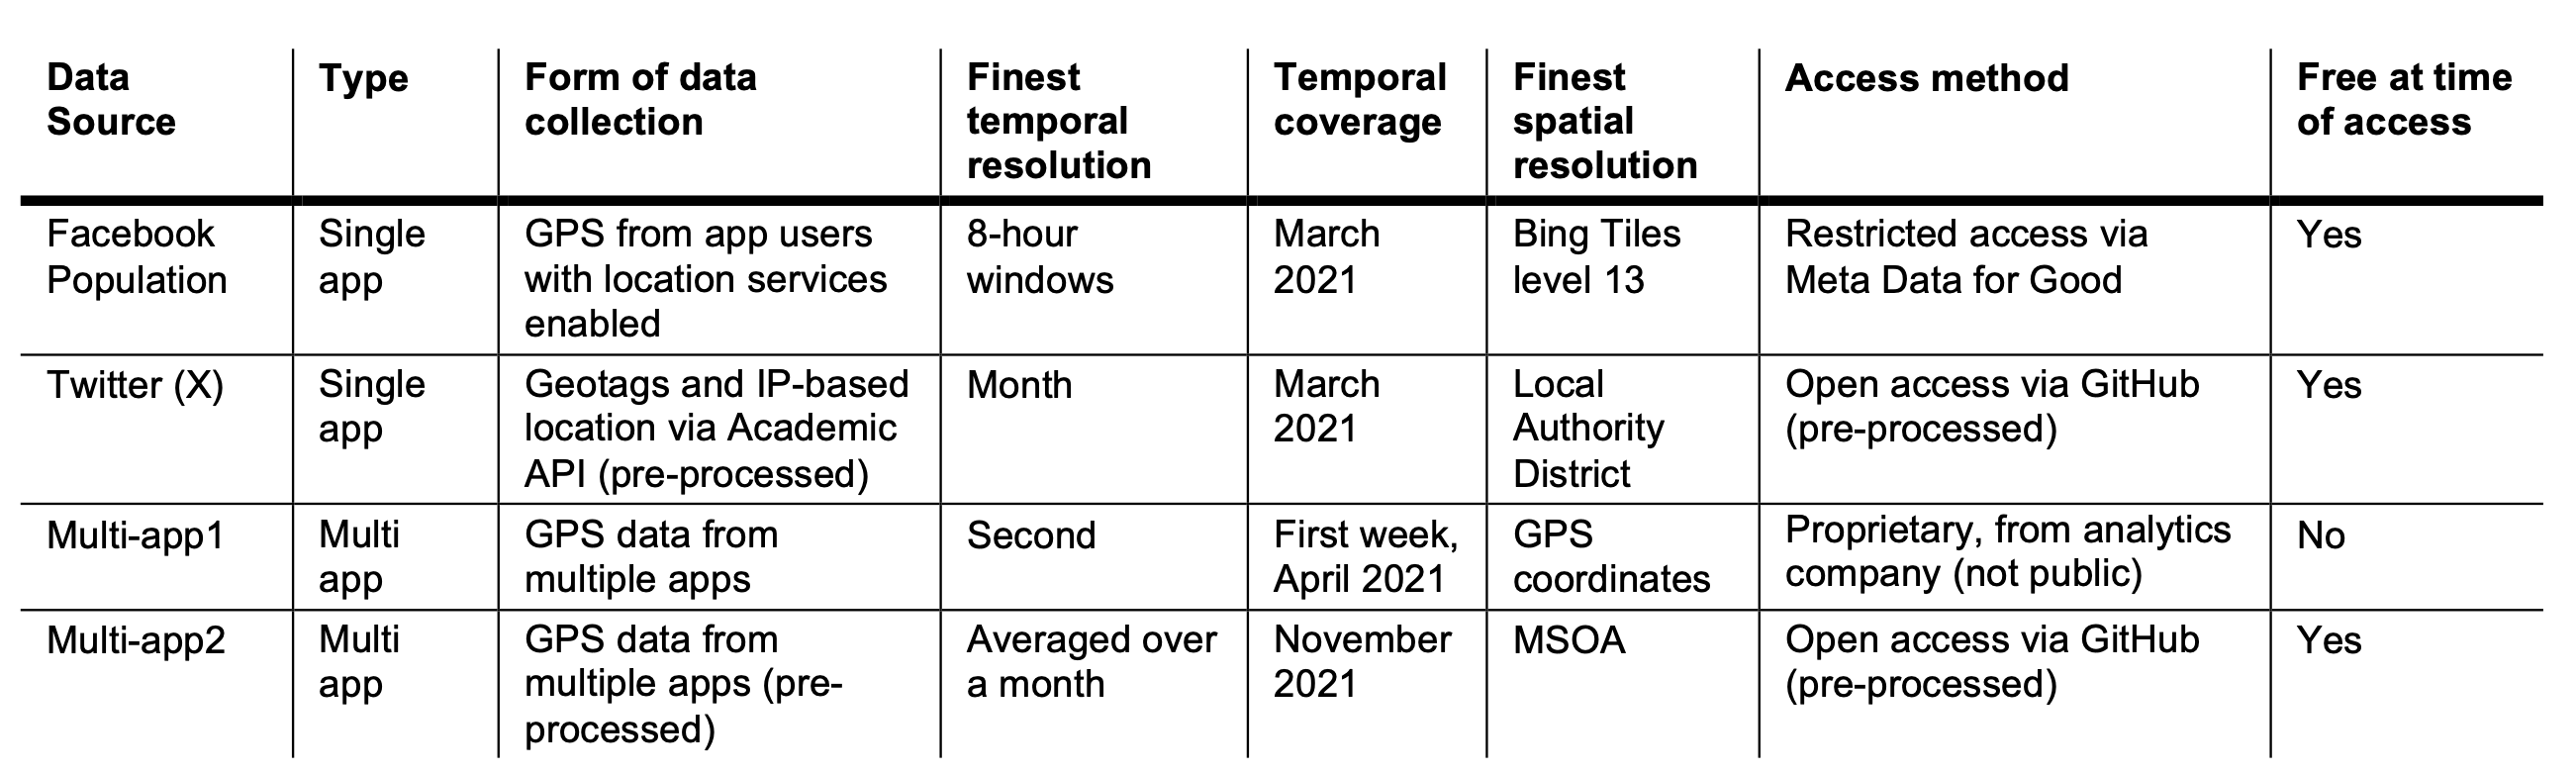
\includegraphics[width=1\linewidth]{figures/table-data-source.png}
\caption{Summary description of mobile phone data sources.}
\label{tab:data-source}
\end{table}

\subsubsection{Meta}\label{meta}

We use the Facebook Population dataset created by Meta and accessed
through their Data for Good Initiative
(\url{https://dataforgood.facebook.com}). This consists of anonymised
aggregate location data from Facebook app accounts in the UK, who have
the location services setting activated. We take the number of unique
accounts as a proxy for the number of unique users, although it could be
the case that one user has more than one account. We selected data
entries covering March 2021, the month when the most recent UK Census
was carried out. Prior to releasing the datasets, Meta ensures privacy
and anonymity by removing personal information and applying several
techniques which include small-count dropping for population counts
under 10, addition of random noise and spatial smoothing using inverse
distance-weighted averaging \citep{maas2019}.

The dataset includes the number of active Facebook app users, aggregated
into three daily 8-hour time windows (i.e.~00:00-08:00, 08:00-16:00 and
16:00- 00:00). To approximate the resident population, we focus on the
time window corresponding to nighttime hours (00:00--08:00), when users
are more likely to be at home. For the study area, this time window
yields an average of 4.2 million daily user records. Spatially, the
Facebook Population data is aggregated according to the Bing Maps Tile
System \citep{bingmaps_tile_system}. In this study, we use data aggregated at
Bing tile level 13, which corresponds to a spatial resolution of
approximately 4.9 \(\times\) 4.9 km at the Equator \citep{maas2019}.

We process the Facebook Population data by averaging daily values and
aggregating them to the level of Local Authority Districts (LADs), to
ensure temporal and spatial alignment with official census data. In the
Supplementary Information, we test alternative processing strategies,
including averaging over a single week in March and reversing the order
of spatial and temporal aggregation. These sensitivity tests confirm
that our main findings are robust to variations in the data processing
workflow.

\subsubsection{Twitter}\label{twitter}

We use an anonymised, analysis-ready dataset of active X (previously
Twitter) accounts in the UK, originally collected via the Twitter
Academic API. Like in the data for Meta, we take the number of unique
accounts as a proxy for the number of unique users. The data consists of
monthly records for the location of unique Twitter accounts, spatially
aggregated across the UK, and is openly available at
\url{https://github.com/c-zhong-ucl-ac-uk/Twitter-Internal-Migration}.
Geolocation is obtained either directly from geotagged tweets or through
manual geocoding using bounding boxes provided by the API, based on the
IP address of the posting device (for methodological details, see
\citep{wang2022}). The full dataset includes approximately 161 million tweets
from February 2019 to December 2021. For this study, we restrict the
analysis to March 2021 to align with the timing of the 2021 UK Census,
during which 125,637 user home locations were identified. Home locations
are assigned to Local Authority Districts (LADs) using a frequency-based
detection algorithm, further described in \citep{wang2022}.

\subsubsection{Multi-app1}\label{multi-app1}

We sourced data from a location analytics company that collects GPS data
from approximately 26\% of smartphones in the UK. The raw data consist of
anonymised device-level GPS traces collected via a range of smartphone
applications, where users have explicitly granted location-sharing
permissions. We consider the number of devices as a proxy for the number
of unique users, although it could be the case that some users have more
than one device. The dataset spans a 7-day period corresponding to the
first week of April 2021 and includes 443,553,155 GPS records. Although
the dataset does not perfectly align with the official 2021 UK Census
date, the temporal proximity ensures a high degree of comparability.

To infer the place of residence of users, we apply a commonly used
rule-based classification method, following approaches outlined in
\citep{wang2022, zhong24working}. Specifically, the place of residence
associated with a device is defined as the location with the highest
number of GPS records recorded during nighttime hours (10 PM--6 AM). To
be classified as a residence, a location must account for more than 50\%
of the device nighttime records. Furthermore, the number of nighttime
records during the observation period must be at least 2. For
comparability across data sources, all identified residence locations
are aggregated to the level of Local Authority Districts (LADs). Using
this method, we detect 1,536,922 home locations.

\subsubsection{Multi-app2}\label{multi-app2}

Our analysis includes a second source of analysis-ready location data,
which is openly-available on GitHub
(\href{https://t.ly/dzlzB}{https://t.ly/dzlzB)}). This dataset has already
been processed to identify the home location of users according to the
methodology described in \citep{zhong24working}. The raw data is collected by
a UK-based data service company, which licenses mobile GPS data from 200
smartphone apps and applies pre-processing methods to ensure user
privacy and anonymity. The dataset covers the entire UK for November
2021 and includes inferred home and work locations for 630,946 users.

While this period does not exactly coincide with the 2021 UK Census, the
difference of less than a year is considered sufficiently close for our
analysis. To ensure consistency across datasets, we further process the
data by aggregating it spatially from the Middle Layer Super Output Area
(MSOA) level to the Local Authority District Level (LAD).

\subsubsection{Census data}\label{census-data}

In addition to the mobile phone app data sources described above, we use
resident population counts from the 2021 UK Census, aggregated at the
LAD level. UK Census is trusted as the official benchmark for population
counts, so we take these as the ground truth for comparing estimates
derived from each digital dataset. We also draw on a set of area-based
covariates from the census, covering demographic, socioeconomic, and
housing characteristics, along with the geographic coordinates of each
LAD centroid. These variables are used to investigate and explain the
contextual factors most strongly associated with the magnitude and
spatial variation of bias in the digital trace data. The full list of
covariates is provided in Table \ref{tab:covariates} .

\begin{table}[h]
\centering
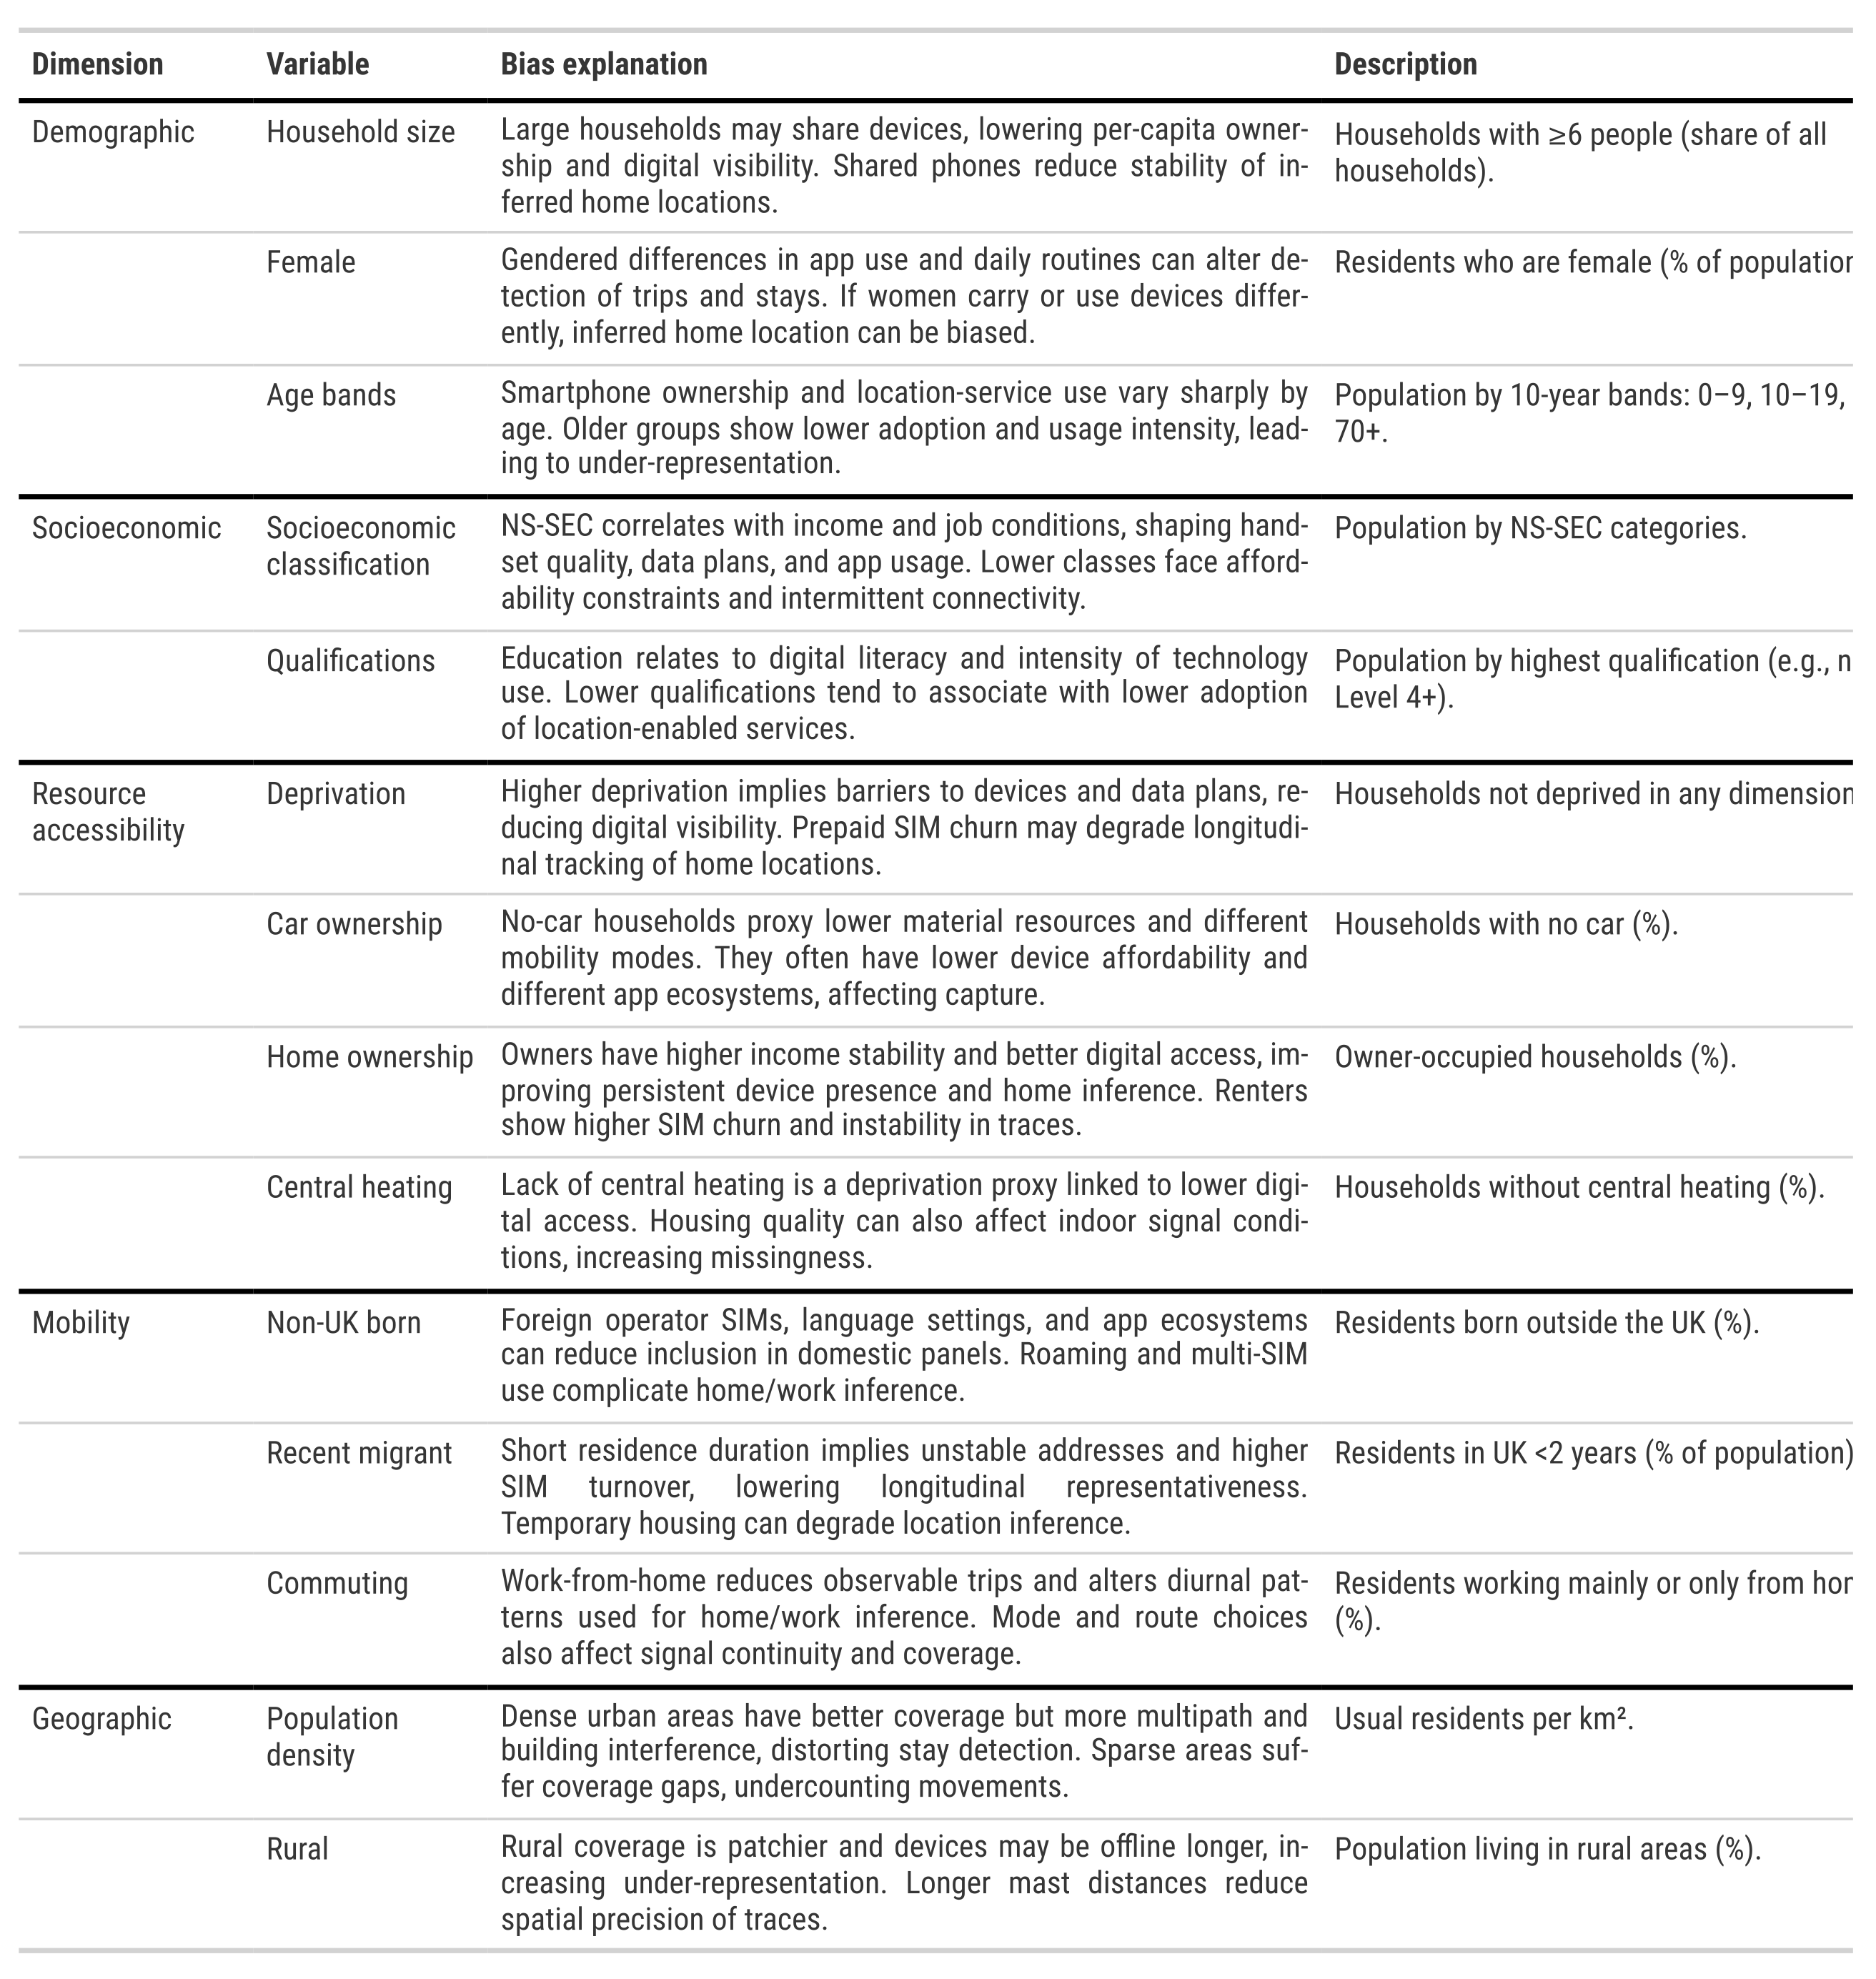
\includegraphics[width=1\linewidth]{figures/01_table-variable-dictionary_explain.png}
\caption{Model variable description, expected influence and description.}
\label{tab:covariates}
\end{table}

\section{Methods}\label{methods}

We introduce a framework to measure and explain biases systematically in
population count data derived from mobile phones (MPs). This framework
consists of three stages. In the first stage, we introduce a metric to
quantify bias related to population coverage within a given geographic
area. In the second stage, we calculate the coverage metric for
different data sources and subnational geographic areas. We then analyse
its variability and assess whether it is evenly distributed across
geographies. Detecting such patterns is important for understanding the
limits of data applicability, and to assess whether spatial dependencies
should be considered in the third stage of the analysis. In the third
stage, we use explainable machine learning to model the variation in
coverage bias as a function of demographic and socioeconomic covariates
derived from the 2021 UK census. This modelling approach allows us to
model the magnitude of bias across areas and, importantly, to quantify
the relative importance of each covariate, so it is possible to identify
the population characteristics (e.g.~age structure, income levels,
educational attainment) that are most strongly associated with
overrepresentation or underrepresentation in the different sources of MP
app data. Figure 1 provides an overview of the methodological workflow,
which includes data acquisition, bias measurement, comparative analysis
with national surveys, spatial analysis, and bias explanation through
modelling.

\subsubsection{Measuring coverage bias}\label{measuring-coverage-bias}

We define a metric to quantify the magnitude of coverage bias in each
subnational area. This metric is based on the population coverage of the
dataset, which we compute as the ratio of the population captured by
dataset \(D\) (sample size) in a geographic area \(i\), denoted as \(P_i^D\),
to the total local population of the same area, \(P_i\). Formally, the
coverage \(c_i\) for area \(i\) is given by: \begin{equation}
c_i = \dfrac{P_i^D}{P_i} \times 100.
\end{equation} The resulting ratio \(c_i\) is assumed to take values
between \(0\) and \(100\), with 100 representing full population coverage.
If users have multiple accounts, the ratio can exceed \(100\), since the
total sample size could be greater than the local population of area
\(i\).

We then define the size of bias \(e_i\) for area \(i\) as:

\begin{equation} \label{eq:size-bias}
e_i = 100 - c_i
\end{equation}

A value of \(e_i = 0\) indicates a lack of coverage bias, which
corresponds to full population coverage (\(c_i = 100\)). We use this bias
indicator to analyse the magnitude and distribution of coverage bias
across multiple sources of data and geographic areas.

\subsubsection{Identifying spatial patterns of population bias}\label{identifying-spatial-patterns-of-population-bias}

For each data source, we compute the coverage bias metric at the
subnational level and examine its geographic variation. This stage has
two main objectives. First, to assess whether bias is evenly distributed
across geographies. Second, to determine whether spatial effects are
sufficiently strong to consider them in the subsequent methodological
stage through the inclusion of spatial lag terms in the explainable
machine learning model.

To evaluate the variability of bias across geographies, we first conduct
exploratory analyses using thematic maps and histograms. To formally
test for spatial clustering, we calculate Moran's I statistic for each
dataset. Because Moran's I is sensitive to the definition of spatial
relationships, we evaluate four alternative spatial weighting schemes:
1) queen neighbourhood, 2) k-nearest neighbours, 3) distance band (set
by algorithm), and 4) distance band (set by user) {[}\textbf{REF}{]}. Comparing
results across these schemes enables us to assess the robustness of
clustering patterns to different neighbourhood definitions. In the main
body of the paper, we report Moran's I values obtained using scheme 1,
as it produces the highest statistic across datasets when statistically
significant, thereby providing the most conservative test for the
presence of spatial clustering. Results for the other schemes are
provided in the Supplementary Information.

Finally, to examine whether bias is associated with population size, we
generate scatterplots comparing population counts from the digital data
sources with census population counts. If bias varies with population
size, we would expect systematic departures from proportionality.
Conversely, an approximately linear relationship through the origin with
a stable slope would suggest that bias is largely independent of
population size. We quantify this relationship by computing Pearson's
correlation coefficient.

\subsubsection{Explainable machine learning}\label{sec-eml}

We used explainable machine learning to identify the key predictors of
population bias and how these the importance of these predictors varies
across geographical areas. Existing evidence based on social media
suggests that population location data from digital platforms are biased
over-representing urban, wealthy and young-adult populations \textbf{{[}REF{]}}.
We therefore modelled our measure of population bias from
Equation\textasciitilde{}\ref{eq:size-bias} as a function of key area-level attributes
reflecting geographical differences in engagement and access to digital
technology across demographic, socioeconomic, household, housing and
location factors. Table 2 reports the set of predictors included in our
analysis. We used data from the 2021 census for England and Wales to
measure these predictors.

We used an eXtreme Gradient Boosting (XGBoost) algorithm. XGBoost is an
ensemble that combines outputs from multiple models to produce a single
prediction and represents an efficient and scalable adaptation of the
gradient boosting machine algorithm proposed by \citep{friedman2001a}. It
utilises gradient descent to improve model performance, and decision
trees are built iteratively, with each tree built to minimise the error
residuals of a preceding iteration. XGBoost has been optimised for
scalability and computational efficiency, providing high predictive
accuracy with limited training time \citep{chen2016, nielsen2016tree}.
XGBoost has also become one of the most widely-used off-the-shelf
machine learning models in applied settings because of its built-in
regularization that mitigates overfitting, sparsity-aware tree
construction and parallelisation efficiency \citep{chen2016}. It can
accommodate nonlinearities and is robust to multicollinearity
\citep{chen2016}. We fitted the following XGBoost regression model.

\begin{equation} \label{eq:xgb-model}
\widehat{e}_i 
= \sum_{m=1}^M f_m\bigl(D_i, S_i, H_i, U_i, L_i\bigr),
\quad f_m \in \mathcal{F}
\end{equation}

\(e_i\) is our measure of population bias. \(f_m\) denotes an individual
regression tree from the boosted ensemble \(\mathcal{F}\) and \(M\) is the
total number of trees. The input variables \(D\), \(S\), \(H\), \(U\), \(L\)
represent key demographic, socioeconomic, housing, household, and
locational attributes of area \(i\), respectively. The model iteratively
learns the contribution of each feature to the prediction of the bias
indicator \(e_i\), allowing for complex, nonlinear interactions.

To implement Equation\textasciitilde{}\ref{eq:xgb-model}, we randomly split the data
into training (80\%) and testing (20\%) sets to ensure robust model
evaluation. We used 10-fold cross validation to train models and
performed grid search over learning rates, tree depths, subsample
ratios, and regularisation penalties to identify optimal
hyperparameters. We applied regularisation penalties including L1
(Lasso) and L2 (Ridge) terms to penalise overly complex trees, promote
feature sparsity, improve model generalisation and mitigate
multicollinearity among predictors. XGBoost's tree-based structure
additionally handles multicollinearity by hierarchically selecting the
most informative splits \citep{chen2016}. We then fitted a final model on the
full training set using these tuned settings of optimal parameters and
evaluated on the held-out test set. We evaluated models based on the
number of trees minimising the root mean squared error (RMSE), the
convergence of training and test error, and difference between predicted
and observed values.

\section{Results}\label{results}

In this section, we illustrate our proposed methodological framework on
four sources of digital data derived from mobile phone (MP) apps. As
described in the Data section, these sources include data for the UK,
collected in or around March 2021 to align as closely as possible with
the reference date of the most recent national census. This temporal
alignment ensures comparability, as the census data serve as the ground
truth against which population counts from the digital sources are
evaluated.

\subsection{The extent of population bias varies across data sources}\label{the-extent-of-population-bias-varies-across-data-sources}

We begin by quantifying coverage bias in each of the mobile phone (MP)
datasets, defined as a function of the proportion of the total
population captured by the dataset, as defined in Equation
\ref{eq:size-bias}. Coverage bias is first computed at the national
level for each MP data source. To contextualise these results, we
compare the MP sources with several widely used traditional datasets,
including major UK surveys available through the UK Data Service
\citep{ukdataserviceSurveysData}. Figure X presents these comparisons across
data sources, showing on the top x-axis the population coverage
(expressed as the number of respondents or subjects per 1,000 people)
and on the bottom x-axis the corresponding measure of coverage bias.

\begin{figure}
\centering
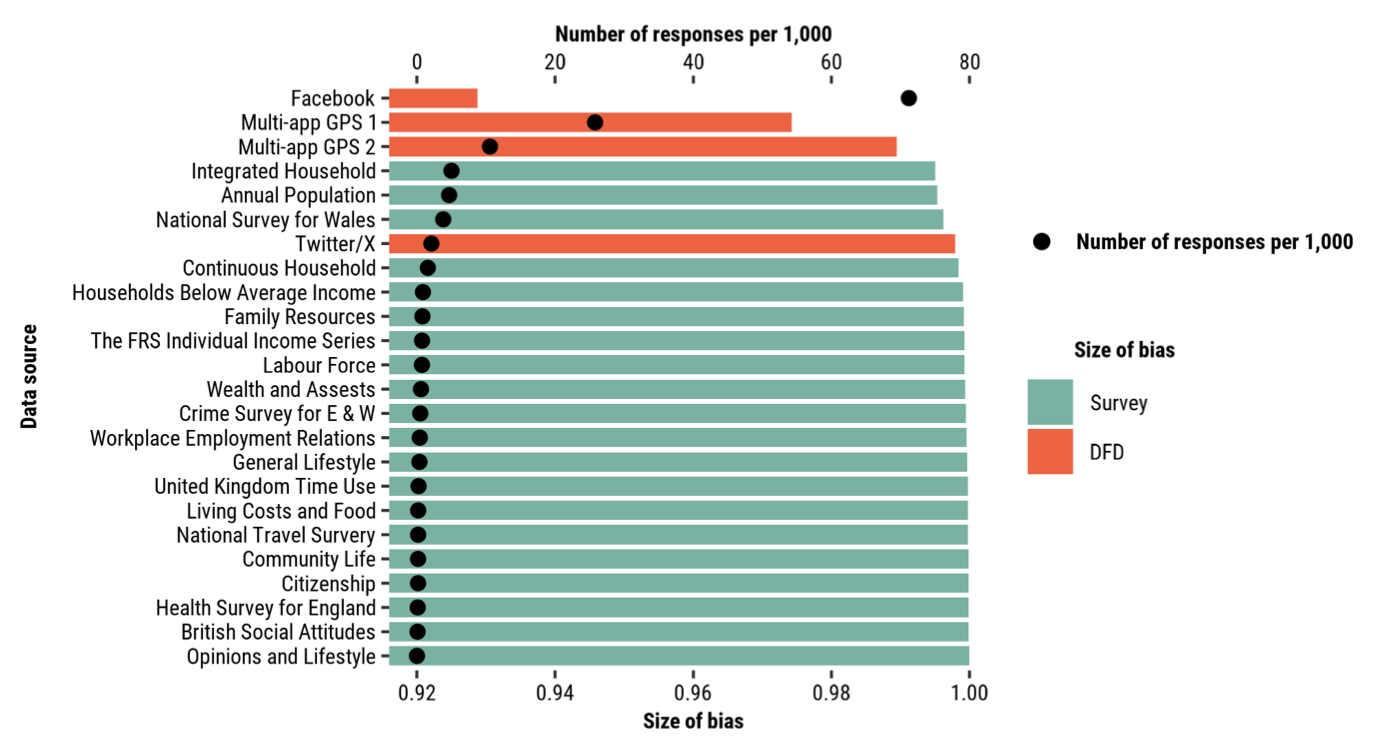
\includegraphics[width=14cm,height=8.5cm]{figures/compare-surveys-legend.png}
\caption{Size of coverage bias (bottom x-axis) and population coverage per 1,000 population (top-x-axis) by data source.}\label{fig:survey}
\end{figure}

Figure \ref{fig:survey} suggests that, with comparatively greater
population coverage and lower coverage bias, MP data have a strong
potential to support large-scale empirical analyses. However, high
population coverage alone does not ensure the data is representative of
different population groups. In surveys, specific strategies are usually
implemented during the data generation process to improve the
statistical representativeness of the sample. For example, sampling
techniques such as stratified sampling or cluster sampling can be
applied so that the sample reflects the broader population of interest.
After sampling, if certain groups remain under-represented, responses
can be adjusted using post-stratification techniques \citep{lohr2021}.
However, even when these strategies are applied, there is no guarantee
that the survey will be fully representative of the broader population
of interest \citep{cochran1977sampling}. This is because representativeness
can only be achieved with respect to a finite set of attributes (e.g.
age, gender, income levels, location, etc.). Ensuring perfect
representativeness would only be possible by surveying the whole
population, which is practically not feasible.

With MP data, achieving statistical representativeness is even more
challenging. Unlike survey data, which is actively collected using
structured sampling methods, MP data is generated passively as a
byproduct of digital interactions, transactions, or device usage,
without any control over who is included in the dataset. Furthermore, by
the time this data reaches researchers or analysts, it is often
anonymised, and does not contain demographic identifiers. As a result,
it is not possible to apply the standard post-stratification weighting
techniques that are typically used to adjust survey or census data for
improved representativeness.

We argue that, even though we do not always have specific demographic
information of the individuals captured through digital trace data, we
can infer some of these characteristics by leveraging the
spatio-temporal granularity of MP data. This is a necessary first step
to understand which population groups might be overrepresented or
underrepresented in different sources of MP data. This information is
necessary to develop subsequent data adjustment strategies that can
improve the representativeness of the data relative to the target
population.

\subsection{Population bias varies widely over space}\label{population-bias-varies-widely-over-space}

We next leverage the fine-grained geographic resolution of the MP app
data sources to examine coverage bias at subnational levels. Analysing
the distribution of coverage bias across geographies allows us to
identify uneven patterns of population coverage across areas and assess
whether these patterns exhibit spatial clustering. On the one hand,
these assessments can help evaluate the limitations in the applicability
of each dataset for further research, and on the other, they inform
whether spatial effects should be incorporated into the subsequent
modelling stage.

Figure \ref{fig:bias-size} shows multiple visualisations that
reflect the distribution of coverage bias at the Local Authority
District (LAD) level. Each row corresponds to a data source and includes
three elements. First, a hexagonal cartogram for the size of coverage
bias in each LAD, representing the LADs as hexagons of equal size to aid
comparability of LADs while maintaining their relative positions. The
maps are presented alongside the associated Moran's I and corresponding
p-value as a measure of spatial autocorrelation. Second, a histogram
showing the statistical distribution of coverage bias across LADs.
Third, a scatter plot comparing the population counts derived from each
of the MP app data sources and the corresponding census population for
each LAD. The scatter plot is accompanied by the Pearson correlation
coefficient and corresponding p-value.

\begin{figure}
\centering
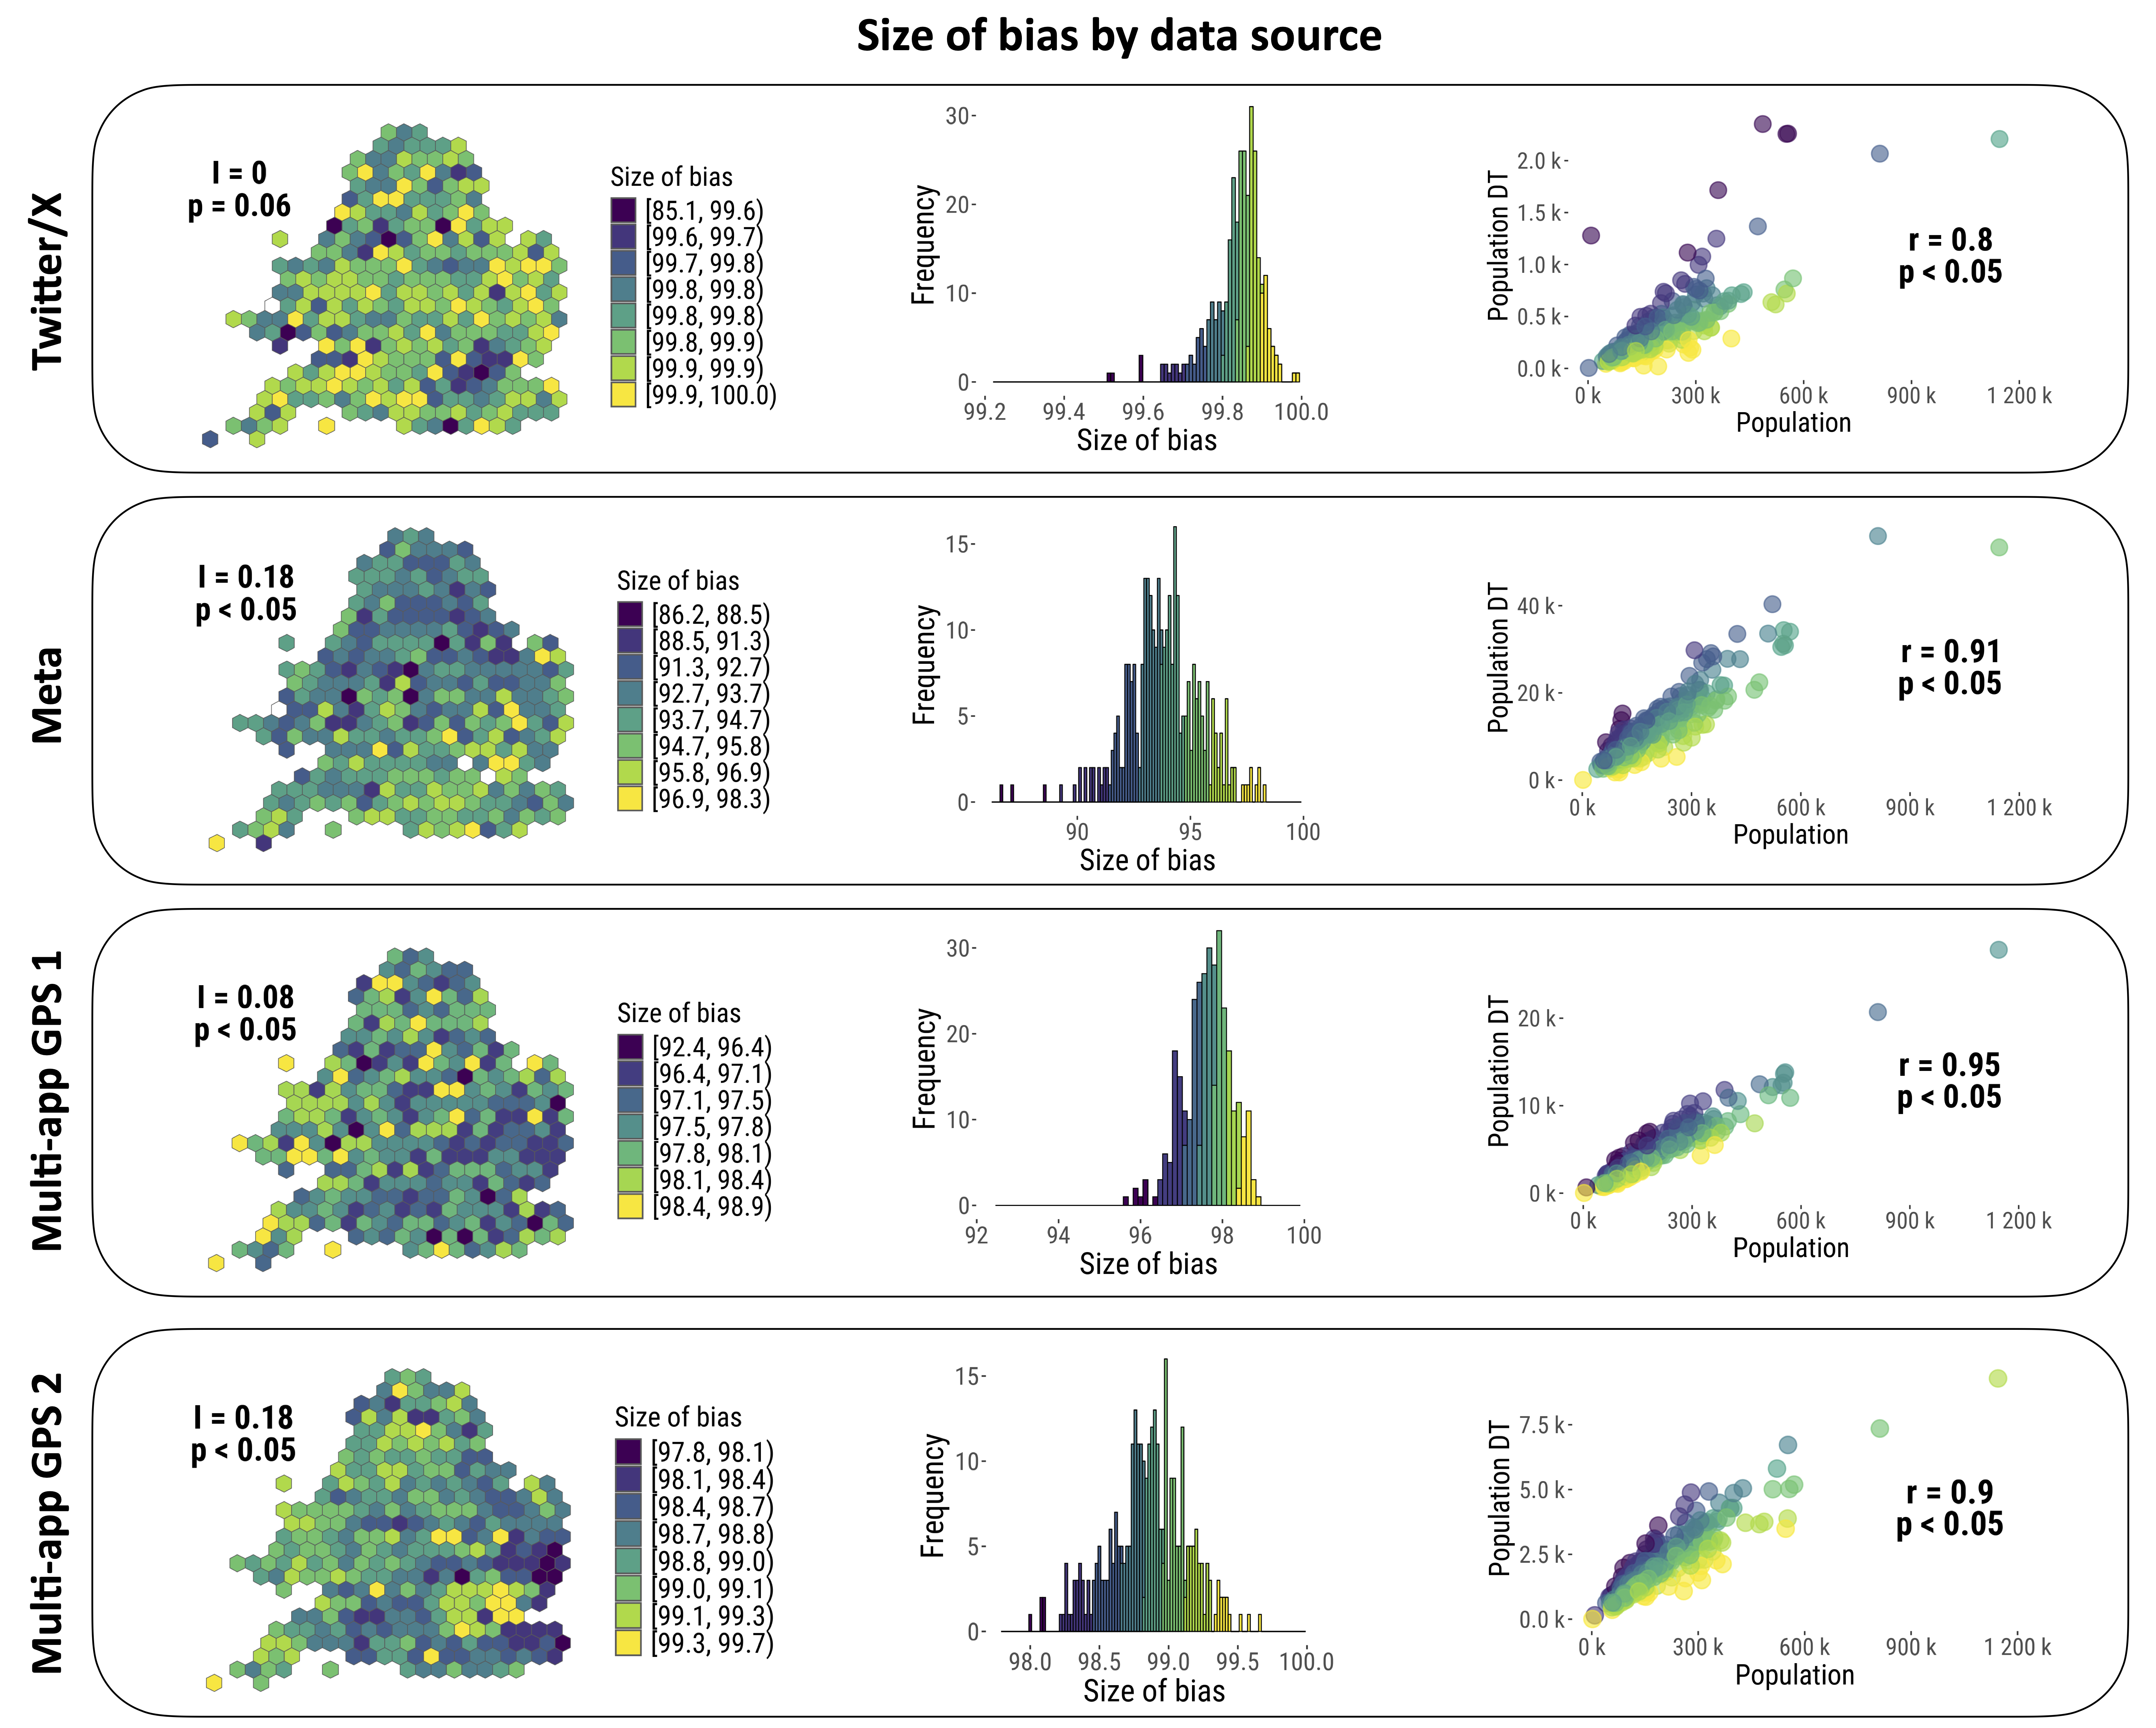
\includegraphics[width=14cm,height=13cm]{figures/Fig-size-bias.png}
\caption{\textbf{Extent and spatial distribution of population bias across local authority districts in the UK.} \textbf{A.} Hexagon map of the size of population bias across local authority districts. \(I\) represents the Moran's I and \(p\) denotes the associated p-value. \textbf{B.} Histogram of the distribution of the size of population bias. \textbf{C.} Scatter plot of the relationship between population size and size of bias.}\label{fig:bias-size}
\end{figure}

Our spatial analysis reveals several patterns in the distribution of
coverage bias which are consistent across the mobile phone (MP)
datasets. First, all data sources exhibit noticeable geographic
variability in coverage bias, as evidenced by the spread of values in
their respective distributions, as displayed in the histograms. This
variability highlights that for a given data source, the degree of
representation can differ substantially between areas.

Second, despite the variability in coverage bias, the maps do not reveal
strong geographic clustering patterns. Bias values fluctuate across
longitude and latitude, and there are no clear north--south or east--west
gradients. This observation is quantitatively supported by the Moran's I
statistics, which are generally statistically significant, but close to
zero. Their small magnitude indicates that spatial clustering is weak at
the LAD scale. Consequently, we conclude that it is unnecessary to
include spatial dependence terms (e.g.~spatial lag) in the subsequent
modelling stage of our framework.

Third, the variability in coverage bias is not explained by the absolute
population size of each subnational unit. Scatter plots comparing
population counts derived from MP app sources and from the census reveal
strong linear relationships. This is quantitatively supported by Pearson
correlation coefficients consistently close to one and statistically
significant.

These findings suggest that coverage bias at the LAD level is not
explained by geographic location or population size, but rather, by
other area-level characteristics such as demographic or socioeconomic
composition. We examine these factors in the third stage of our analysis.

\subsection{Key contextual features explain population biases}\label{key-contextual-features-explain-population-biases}

We assessed the contribution of key contextual features to explaining spatial variations in population biases across demographic, socioeconomic, resource accessibility, mobility and geographic domains. Figure \ref{fig:radialplots} displays the relative importance of each individual model feature, representing the average absolute SHapley Additive exPlanations (SHAP) value per feature including in our XGBoost model described in Section \ref{sec-eml} \textbf{{[}REF{]}}. SHAP values are standardised by data source based on minimum and maximum scores to enable comparability. Figure \ref{fig:radialplots} highlights features with standardised importance scores over 0.5 for individual data source.

\begin{figure}
\centering
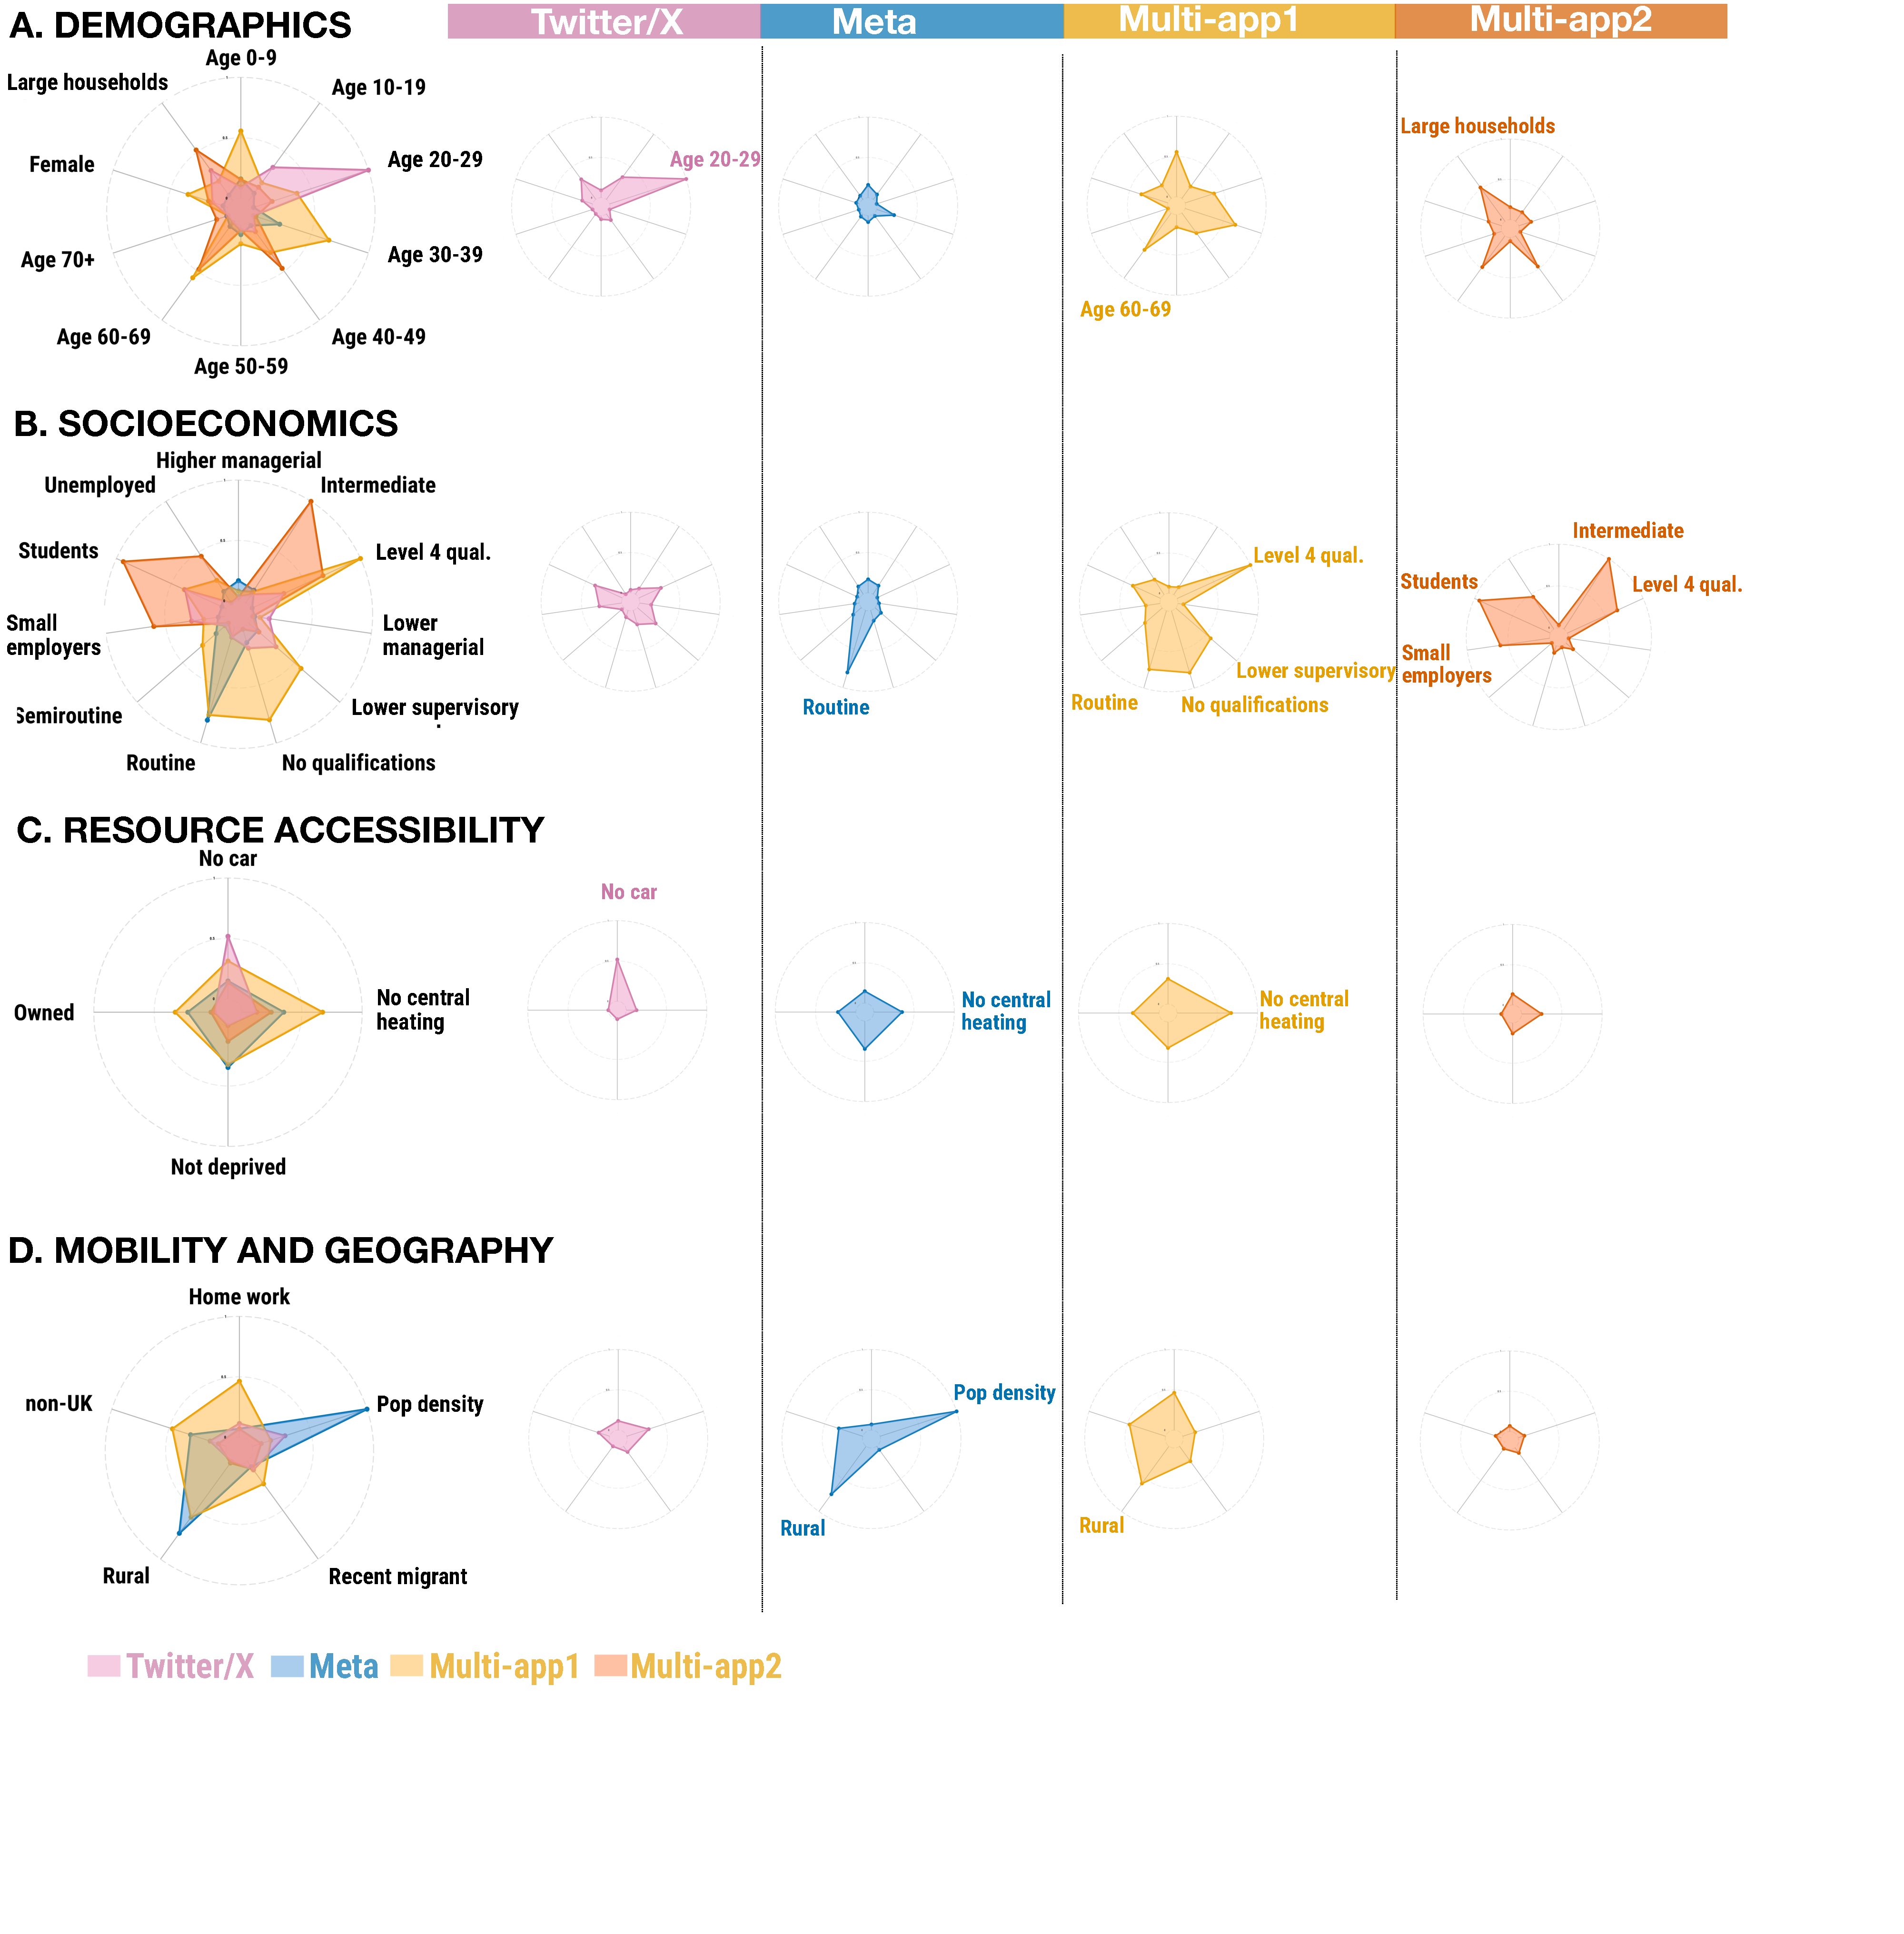
\includegraphics[width=14.2cm,height=15.8cm]{figures/radial-plots_feature-importance.png}
\caption{\textbf{Radial charts illustrating the importance of, and contribution to, explaining differences in population biases across local authority districts.} The importance is estimated based on SHAP feature importance scores, calculated as the average absolute SHAP value per feature using an XGBoost machine learning algorithm. Average absolute SHAP values were normalised across individual data using minimum and maximum scores, to ensure comparability across data sources. First column displays the estimates for all data sources and model features. Subsequent columns highlight features scoring SHAP values over 0.5 within a 0-1 range for individual data sources.}\label{fig:radialplots}
\end{figure}

The results reveal wide variability in the key predictors of population biases across digital data sources. Demographic and socioeconomic features appear as the most important predictors of population bias in Twitter/X data. Two features standout -the shares of population aged 20-29 and no car ownership- reflecting the over-representation of the young adult populations or population with access to resources on active Twitter/X users. In addition to demographic and socioeconomic features, resource accessibility and geographic attributes also display some of the largest contributions to explain population biases across Meta, Multi-app1 and Multi-app2 platforms. Coupled to the share of population in routine occupations and lacking central heating, geographical factors particularly population density and rurality report the highest SHAP averages, contributing to explain the spatial variability of Meta-derived population biases. Socioeconomic features standout as the most important predictors of population biases across both multi-app platforms, though differences exist. The population share with high or no qualification, and working in low skill occupations emerge as the most important features in explaining population biases in Multi-app1. This is in addition to the population share aged 60-69, residing in households lacking central heating and living in rural areas. For multi-app2-derived estimates, the share of student population, working in intermediate-level jobs, small employers, having a Level 4 qualification and living in large households score the highest average SHAP values. The variability in feature importance ranking across data sources reflects differences in the contextual features that contribute to explaining biases in their respective population estimates.

\begin{figure}
\centering
\includegraphics[width=14.1cm,height=12.2cm]{figures/explain-bias.png}
\caption{\textbf{Top ranked model features contributing to explaining population biases across local authority districts from an XGboost model.} (a) beeswarm plots of SHAP feature values displaying the relative importance and direction of influence of the top 20 contextual features on the extent of population bias. Features are ranked by their mean absolute SHAP value, with colours indicating feature values (low to high). (b) SHAP dependence plots for the top six features based on their mean absolute SHAP value, illustrating the marginal effect of variation in each predictor on population bias. Local polynomial regression modelling was used to represent local trends with 95\% confidence intervals. Each point represents a local authority district.}\label{fig:shap-plots}
\end{figure}

Expanding this evidence, Figure \ref{fig:shap-plots} depicts the way these contextual features contribute to increasing or reducing the extent of population bias across LADs. Figure \ref{fig:shap-plots}.a shows the top 20 features based on their average SHAP value from the highest to the lowest. Figure \ref{fig:shap-plots}.b displays top six of these features revealing how changes in feature values contribute to changes in population bias, with colour encoding feature values. For instance, the first column of plots show that areas with larger shares of population aged 20-29 and lacking central heating tend to have lower population bias compared to those with larger shares in Twitter/X-derived estimates. In contrast, areas with larger shares of population aged 10-19 are associated with higher Twitter/X-based population bias, potentially reflecting a limited number of active Twitter/X users in this age range. Of the features highlighted in Figure \ref{fig:radialplots}, Figure \ref{fig:shap-plots} indicates that population estimates derived from Meta tend to have larger biases in areas with higher population density and greater percentages of people lacking central heating. Operating in the opposite direction, larger shares of people working in routine-level jobs and living in rural areas display lower Meta-based population bias, reflecting greater engagement with Facebook among these communities. For multi-app1-derived estimates, biases are larger for areas with greater shares of population with Level 4 or no qualification, working in routine-level jobs, lacking central heating, living in rural communities and population aged 60-69. For multi-app2-derived estimates, biases are greater for areas with smaller shares of people working in intermediate-level jobs and self-employed in small businesses, but displaying larger percentages of students, people with Level 4 qualification and living in large households.

Figure \ref{fig:shap-plots} also reveals systematic complex nonlinear shapes in the association between contextual features and population bias. We identified three types of nonlinear relationships. First is curvilinear associations in the way of U-shape or inverse U shapes. These involve patterns of population biases decreasing at low values of contextual features, increasing at medium values and reducing again - or the reverse. A distinctive pattern of these associations is their curvature representing a reversal in the direction of the relationship between population bias and a contextual feature. Meta-based population density and Multi-app2-based intermediate feature estimates represent prominent curvilinear relationships. A second pattern takes the form of S-shaped associations. The distinctive feature of these associations is their multiple phase composition displaying a different pattern of population biases at
low and high end values of the contextual feature relative to middle range feature values. Twitter/X-based 20-29 age estimates, for example, display high and unchanging population bias at low feature values, highly variable bias at mid values and low but increasing population bias at high values. A third pattern is threshold/stepwise associations representing sharp changes at a cut-off. The distinctive feature of this pattern is sharp ``steps'' or thresholds where the relationship between population bias and a contextual feature changes abruptly. Population biases would remain flat at low values and then jump and plateau at higher values. Our Multi-app1 estimates for Level 4 qualification represent a clear illustrative of this type of association displaying flat small population bias at low feature values but, then jump and remain high at higher feature values. These shapes do not appear to be data source specific and vary in unpredictable ways across variables.

\section{Discussion}\label{discussion}

\subsection{Key findings}\label{key-findings}

\begin{itemize}
\tightlist
\item
\item
\item
\end{itemize}

\subsection{Implications}\label{implications}

\begin{itemize}
\tightlist
\item
\item
\end{itemize}

\subsection{Challenges and limitations}\label{challenges-and-limitations}

For multi-app - wider set of factors contribute to explaining biases

\begin{itemize}
\tightlist
\item
  Age structure has less predictive importance than socioeconomic and geographic factors\\
\end{itemize}

\section{Conclusion (CC)}\label{conclusion-cc}

\ethics{Please provide details on the ethics.}

\dataccess{Please provide details on the data availability.}

\aucontribute{Please provide details of author contributions here.}

\competing{Please declare any conflict of interest here.}

\funding{Please provide details on funding}

\disclaimer{Please provide disclaimer text here.}

\ack{Please include your acknowledgments here, set in a single paragraph. Please do not include any acknowledgments in the Supporting Information, or anywhere else in the manuscript.}

\bibliographystyle{RS}
\bibliography{sample.bib}


\end{document}
